\section{Funções sobrejetoras, injetoras e bijetoras}

\begin{frame}[allowframebreaks]{Funções sobrejetoras}
    \begin{itemize}
        \item Uma função $f: A \rightarrow B$ é sobrejetora se, e somente se, $Im(f) = B$.

        \item Formalmente têm-se, dado que $f$ é uma função, $f: A \rightarrow B$ é sobrejetora se, e somente se, $\forall y \in B$, $\exists x \in A \mid f(x) = y$.

        \begin{multicols}{2}
            \begin{figure}
            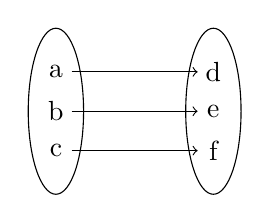
\begin{tikzpicture}
                \draw (0,0) ellipse (10pt and 30pt);
                \draw (2,0) ellipse (10pt and 30pt);
    
                \draw node at (0, 0.5) {a};
                \draw node at (0, 0) {b};
                \draw node at (0, -0.5) {c};
    
                \draw node at (2, 0.5) {d};
                \draw node at (2, 0) {e};
                \draw node at (2, -0.5) {f};
    
                \draw [->] (0 + 0.2, 0.5) -- (2 - 0.2, 0.5);
                \draw [->] (0 + 0.2, 0) -- (2 - 0.2, 0);
                \draw [->] (0 + 0.2, -0.5) -- (2 - 0.2, -0.5);
            \end{tikzpicture}
            \caption{É sobrejetora}
            \end{figure}

            \begin{figure}
            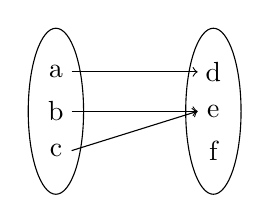
\begin{tikzpicture}
                \draw (0,0) ellipse (10pt and 30pt);
                \draw (2,0) ellipse (10pt and 30pt);
    
                \draw node at (0, 0.5) {a};
                \draw node at (0, 0) {b};
                \draw node at (0, -0.5) {c};
    
                \draw node at (2, 0.5) {d};
                \draw node at (2, 0) {e};
                \draw node at (2, -0.5) {f};
    
                \draw [->] (0 + 0.2, 0.5) -- (2 - 0.2, 0.5);
                \draw [->] (0 + 0.2, 0) -- (2 - 0.2, 0);
                \draw [->] (0 + 0.2, -0.5) -- (2 - 0.2, 0);
            \end{tikzpicture}
            \caption{Não é sobrejetora}
            \end{figure}
        \end{multicols}
    \end{itemize}
\end{frame}

\begin{frame}[allowframebreaks]{Funções injetoras}
    \begin{itemize}
        \item Uma função $f: A \rightarrow B$ é injetora se, e somente se, cada $x$ encontra um $y$ e os elementos distintos possuem imagens distintas.

        \item Formalmente têm-se, dado que $f$ é uma função, $f: A \rightarrow B$ é injetora se, e somente se, $\forall x_1, x_2 \in A, f(x_1) = f(x_2) \Rightarrow x_1 = x_ 2$.

        \begin{multicols}{2}
            \begin{figure}
            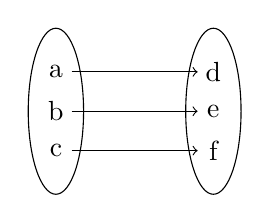
\begin{tikzpicture}
                \draw (0,0) ellipse (10pt and 30pt);
                \draw (2,0) ellipse (10pt and 30pt);
    
                \draw node at (0, 0.5) {a};
                \draw node at (0, 0) {b};
                \draw node at (0, -0.5) {c};
    
                \draw node at (2, 0.5) {d};
                \draw node at (2, 0) {e};
                \draw node at (2, -0.5) {f};
    
                \draw [->] (0 + 0.2, 0.5) -- (2 - 0.2, 0.5);
                \draw [->] (0 + 0.2, 0) -- (2 - 0.2, 0);
                \draw [->] (0 + 0.2, -0.5) -- (2 - 0.2, -0.5);
            \end{tikzpicture}
            \caption{É injetora}
            \end{figure}

            \begin{figure}
            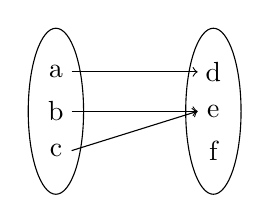
\begin{tikzpicture}
                \draw (0,0) ellipse (10pt and 30pt);
                \draw (2,0) ellipse (10pt and 30pt);
    
                \draw node at (0, 0.5) {a};
                \draw node at (0, 0) {b};
                \draw node at (0, -0.5) {c};
    
                \draw node at (2, 0.5) {d};
                \draw node at (2, 0) {e};
                \draw node at (2, -0.5) {f};
    
                \draw [->] (0 + 0.2, 0.5) -- (2 - 0.2, 0.5);
                \draw [->] (0 + 0.2, 0) -- (2 - 0.2, 0);
                \draw [->] (0 + 0.2, -0.5) -- (2 - 0.2, 0);
            \end{tikzpicture}
            \caption{Não é injetora}
            \end{figure}
        \end{multicols}
    \end{itemize}
\end{frame}